\documentclass[10pt]{article}

\usepackage[letterpaper,margin=1in]{geometry}
\usepackage[T1]{fontenc}
\usepackage{lmodern}
\usepackage{microtype}
\usepackage{amsmath,amssymb}
\usepackage{booktabs}
\usepackage{graphicx}
\usepackage[numbers]{natbib}
\usepackage{hyperref}
\usepackage{xcolor}
\hypersetup{colorlinks=true,linkcolor=black,citecolor=blue,urlcolor=blue}

\title{\vspace{-1.5em}\textbf{SINDy-KAN: Discovering Nonlinear Financial PDEs\\
from Option Market Data}\vspace{-0.4em}}
\author{Makar Ulesov \\ Mohamed bin Zayed University of Artificial Intelligence (MBZUAI) \\
\texttt{makar.ulesov@mbzuai.ac.ae}}
\date{}

\begin{document}
\maketitle
\vspace{-2em}

\begin{abstract}
Discovering the partial differential equations governing option prices directly from market data requires handling noisy derivatives and nonlinear dynamics that lie outside classical model families.
We propose \textbf{SINDy-KAN}, a two-stage framework that uses sparse regression (SINDy) to identify active PDE terms from a candidate library, then trains a Kolmogorov--Arnold Network (KAN) to learn the nonlinear operator on those terms.
Gaussian Process derivative estimation with analytical kernel derivatives extends the practical noise tolerance from under $1\%$ to over $10\%$ ($R^2(\text{clean}){=}0.920$ at $10\%$ noise versus $-0.486$ for finite differences).
On $1{,}374$ real option contracts across SPY, QQQ, AAPL, and MSFT, a $[2,1]$ KAN-Dupire architecture with two learned univariate activations achieves $R^2$ up to $0.925$, compared to $0.604$ for linear Dupire regression, with the diffusion activation revealing the volatility smile as a PDE-level nonlinearity.
The framework also serves as a misspecification diagnostic, detecting jump dynamics on synthetic Merton data via spurious-term activation.
\end{abstract}

\section{Introduction}

Financial derivatives pricing relies on partial differential equations --- Black--Scholes \citep{blackscholes1973}, Dupire \citep{dupire1994pricing}, Heston \citep{heston1993closed} --- whose assumptions often fail on real chains. Data-driven PDE discovery via SINDy \citep{brunton2016sindy,rudy2017pde} has succeeded in physics but faces two challenges in finance: option data is noisy (bid--ask spreads, discrete strikes, interpolation artifacts) which corrupts numerical derivatives, and real market dynamics are nonlinear (the volatility smile, jumps, hedging friction) which a fixed linear candidate library cannot capture.

The closest prior work is Feng et al.\ \citep{feng2025feynmankac} (NeurIPS 2025 Workshop), which recovers a stochastic BSDE from single-stock AAPL trajectories via stochastic SINDy under the risk-neutral measure. We instead discover deterministic PDEs from cross-sectional option \emph{surfaces} and address the nonlinearity challenge by composing SINDy with a Kolmogorov--Arnold Network \citep{liu2025kan}. Mesh-free neural-autograd SINDy \citep{gao2025meshfree} replaces finite differences with autograd through an MLP for physics PDEs; we show below that an analytical Gaussian Process derivative dominates that route on financial data where derivative quality is the bottleneck.

\textbf{Contributions.} (1) The \textbf{SINDy-KAN framework}: SINDy identifies PDE structure, a $[2,1]$ KAN learns the nonlinear operator on the identified terms, achieving $R^2$ up to $0.925$ on real option data versus $0.604$ for linear Dupire regression. (2) \textbf{GP derivative estimation} for financial PDE discovery: analytical kernel derivatives extend noise tolerance from $<\!1\%$ to $>\!10\%$, outperforming five alternative methods on a systematic comparison using $R^2(\text{clean})$. (3) \textbf{Misspecification diagnostic}: SINDy detects jump dynamics on synthetic Merton data via spurious-term activation, validated by a hard-constraint PINN that reduces put pricing relative $L^2$ error from $48.0\%$ to $4.98\%$.

\section{Method}

\paragraph{2.1 Problem setup.} In log-moneyness coordinates $k{=}\log(K/F(\tau))$ with forward $F(\tau){=}S_0 e^{(r{-}q)\tau}$, the Dupire equation reads $\partial_\tau C \;=\; c_1\,\partial_k C \;+\; c_2\,\partial_{kk} C$, where under constant-$\sigma$ Black--Scholes the true coefficients are $c_1{=}-(r{-}q{-}\tfrac12\sigma^2)$ and $c_2{=}\tfrac12\sigma^2$. We construct $C(k,\tau)$ by fitting a per-expiration SVI parameterization \citep{gatheral2014arbitrage} to observed implied volatilities and use the analytical Black--Scholes theta $\theta_i{=}\tfrac{S_0\phi(d_1)\sigma_{\text{imp},i}}{2\sqrt{\tau_i}}{+}rK_i e^{-r\tau_i}N(d_2)$ as the regression target. This replaces a finite-difference $\partial_\tau C$ across $\le 10$ discrete expirations --- the dominant noise source in cross-sectional Dupire discovery (Appendix~\ref{app:tau-fix}).

\paragraph{2.2 GP derivative estimation.} We fit $C(k,\tau)\sim\mathcal{GP}(0,\kappa)$ with an anisotropic RBF or Matern-$5/2$ kernel learned via marginal likelihood maximization, then read off $\partial_k C$ and $\partial_{kk} C$ as conditional means of derivative-augmented kernels \citep{rasmussen2006gp}. This avoids numerical differentiation entirely and moves $R^2(\text{clean})$ from $0.405$ (FD) to $0.951$ (GP) at $5\%$ noise on synthetic Black--Scholes (Table~\ref{tab:noise}).

\paragraph{2.3 SINDy-KAN framework.} \textbf{Stage 1.} STLSQ sparse regression on the GP-derived library $\{C,\partial_k C,\partial_{kk}C,k\partial_k C,k^2\partial_{kk}C\}$ identifies the active terms. On synthetic constant-$\sigma$ data this correctly selects the 2-term Dupire structure with $R^2{>}0.99$. \textbf{Stage 2.} The SINDy-selected active terms become the inputs to a single-layer KAN. For Dupire this is a $[2,1]$ KAN
\[\partial_\tau C \;=\; \phi_{\text{drift}}(\partial_k C) \;+\; \phi_{\text{diff}}(\partial_{kk} C),\]
where each $\phi_i$ is a learned univariate B-spline activation \citep{liu2025kan,koenig2024kanodes}. Under constant-$\sigma$ Black--Scholes both activations are straight lines (with slopes $c_1$ and $c_2$); on real data, nonlinearity in $\phi_{\text{diff}}$ directly reveals the local-volatility structure as a function of the option surface's strike-convexity.

\paragraph{2.4 PINN validation.} We validate discovered PDEs with a hard-constraint physics-informed neural network whose trial function $V(S,t){=}(T{-}t)\,N(S,t){+}\text{payoff}(S)$ guarantees the terminal condition exactly. This drops the put-option relative $L^2$ from $48.04\%$ to $4.98\%$ (Appendix~\ref{app:pinn}).

\section{Experiments}

\subsection{Derivative method comparison}

Table~\ref{tab:noise} reports $R^2(\text{clean})$ for four derivative estimators at representative noise levels on the synthetic Black--Scholes call surface ($r{=}0.05$, $\sigma{=}0.2$, $K{=}100$, $100{\times}100$ grid). Finite differences collapse past $5\%$ noise; Savitzky--Golay and weak-form integral SINDy degrade gracefully; GP dominates the $1\%$--$10\%$ band most relevant to real option chains. Beyond $15\%$, GP's smoothing kernel begins to over-regularize and the weak-form is the only survivor. Figure~\ref{fig:noise} plots the full 13-point sweep with a zoom on the low-noise region.

\begin{table}[h]
\centering\footnotesize
\caption{$R^2(\text{clean})$ by derivative estimator and noise level (synthetic BS, $100{\times}100$ grid). Source: \texttt{all\_methods\_noise\_comparison\_v2.csv}, \texttt{gp\_noise\_robustness.csv}.}
\label{tab:noise}
\begin{tabular}{lrrrrrr}
\toprule
Method & $0\%$ & $1\%$ & $5\%$ & $10\%$ & $20\%$ & $30\%$ \\
\midrule
FD             & $1.000$ & $0.816$ & $0.405$ & $-0.486$ & $-1.298$ & $-1.797$ \\
SavGol         & $1.000$ & $0.958$ & $0.846$ & $0.816$  & $0.650$  & $0.345$ \\
Weak           & $0.901$ & $0.898$ & $0.885$ & $0.888$  & $\mathbf{0.832}$ & $\mathbf{0.572}$ \\
\textbf{GP}    & $\mathbf{1.000}$ & $\mathbf{0.990}$ & $\mathbf{0.951}$ & $\mathbf{0.920}$ & $-0.286$ & $-0.974$ \\
\bottomrule
\end{tabular}
\end{table}

\begin{figure}[h]
\centering

\includegraphics[width=0.78\linewidth]{figures/fig2_noise_robustness.pdf}
\caption{$R^2(\text{clean})$ vs.\ noise across four derivative estimators. GP dominates the $[1\%,10\%]$ band; weak-form integral SINDy is the only survivor at $>\!15\%$. Inset zooms on the low-noise crossover.}
\label{fig:noise}
\end{figure}

\subsection{SINDy-KAN on real option data}

Table~\ref{tab:sindy-kan} is the main empirical result. The $[2,1]$ KAN-Dupire lifts in-sample $R^2$ by $+0.32$ to $+0.47$ over the linear Dupire regression on all four tickers, reaching $R^2{=}0.925$ on MSFT and $0.795$ on SPY (the densest chain). The diffusion-edge linear-fit $R^2$ is $0.83$--$0.96$ on real data versus $\ge\!0.99$ on synthetic constant-$\sigma$ Black--Scholes, confirming the real-data activation is genuinely nonlinear and not an artifact of architecture. The drift edge remains close to linear (lin $R^2{\approx}0.68$) across tickers, consistent with the canonical $-(r{-}q{-}\tfrac12\sigma^2)$ Black--Scholes drift.

\begin{table}[h]
\centering\footnotesize
\caption{$[2,1]$-KAN-Dupire vs.\ linear Dupire on real chains (SVI-smoothed surface, analytical-$\theta$ target). $\Delta$ is in-sample $R^2$ lift; $\phi_{\text{diff}}$ lin $R^2$ measures how nonlinear the diffusion activation is (lower = more nonlinear). Source: \texttt{sindy\_kan\_dupire\_real.csv}.}
\label{tab:sindy-kan}
\begin{tabular}{lrrrrr}
\toprule
Ticker & $n$ opts & Linear Dupire $R^2$ & $[2,1]$ KAN-Dupire $R^2$ & $\Delta$ & $\phi_{\text{diff}}$ lin $R^2$ \\
\midrule
SPY   & $542$ & $0.439$ & $\mathbf{0.795}$ & $+0.356$ & $0.829$ \\
QQQ   & $416$ & $0.401$ & $\mathbf{0.868}$ & $+0.467$ & $0.885$ \\
AAPL  & $244$ & $0.432$ & $\mathbf{0.893}$ & $+0.461$ & $0.925$ \\
MSFT  & $172$ & $0.604$ & $\mathbf{0.925}$ & $+0.321$ & $0.958$ \\
\bottomrule
\end{tabular}
\end{table}

\begin{figure}[h]
\centering
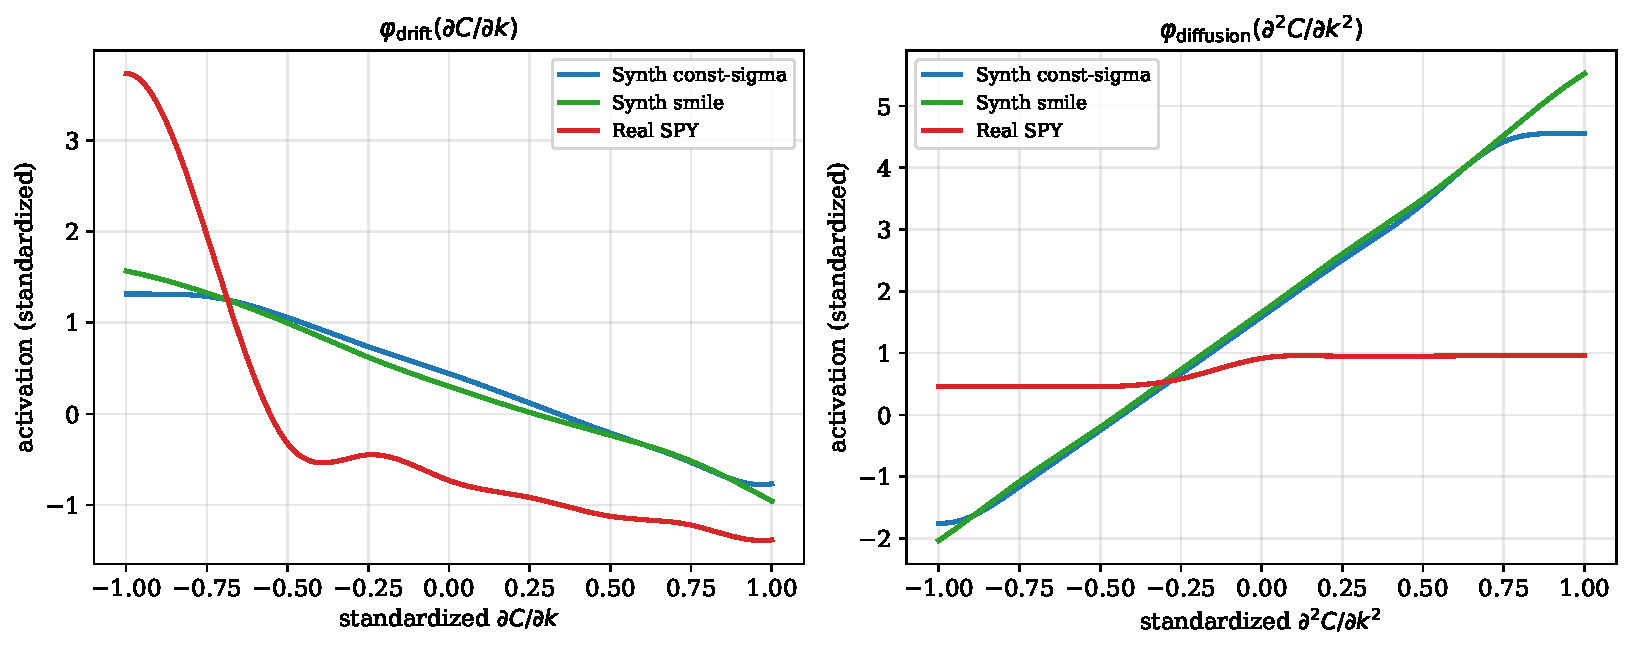
\includegraphics[width=\linewidth]{figures/sindy_kan_activations.pdf}
\caption{$[2,1]$-KAN-Dupire activations. Left: $\phi_{\text{drift}}(\partial_k C)$. Right: $\phi_{\text{diff}}(\partial_{kk} C)$. Blue = synthetic constant-$\sigma$ Dupire (linear, as theory predicts); green = synthetic smile $\sigma^2(k){=}0.04{+}0.10 k^2$; red = real SPY. The diffusion activation deviates from linearity on all four tickers (Table~\ref{tab:sindy-kan}); the shape of the red curve carries the volatility smile as a PDE-level nonlinearity.}
\label{fig:sindy-kan}
\end{figure}

The analytical-$\theta$ choice is what makes the framework work on real data. Replacing finite-difference $\partial_\tau C$ (across $\le 10$ irregular expirations) with the BS theta formula evaluated pointwise from each grid point's SVI-implied $\sigma_{\text{imp}}$ lifts the linear-Dupire $R^2$ from $-0.03$ (FD) to $+0.56$ (analytical) on SPY before any KAN is introduced --- a $\sim\!0.6$ absolute jump driven entirely by the regression target (Appendix~\ref{app:tau-fix}). Bootstrap $95\%$ CI widths contract from $\sim\!0.085$ to $\{0.016,0.019,0.020,0.030\}$ over the four tickers.

\subsection{Misspecification detection}

Table~\ref{tab:merton} reports a SINDy fit with the Black--Scholes library on synthetic Merton jump-diffusion data. The Black--Scholes-canonical $V$, $S\partial_S V$, $S^2\partial_{SS} V$ terms recover values close to their BS counterparts, but the spurious $\partial_{SS} V$ coefficient (true value $0$ under BS) is identified as $\mathbf{1.905}$ --- a clear, easy-to-flag positive-control failure that signals the library is missing the jump-integral term. A Heston variance-slicing experiment recovers the linear $\sigma^2$ scaling of the diffusion coefficient with slope $-0.5001$ (true: $-0.500$), matching the Heston structure to four decimals (Appendix~\ref{app:heston}).

\begin{table}[h]
\centering\footnotesize
\caption{SINDy on synthetic Merton jump-diffusion data with the BS library. $\partial_{SS}V$ is the misspecification flag (true value $0$ under BS). Source: \texttt{merton\_discovery.csv}.}
\label{tab:merton}
\begin{tabular}{lrr}
\toprule
Term & BS truth & Merton-fit \\
\midrule
$V$              & $+0.0500$ & $+0.0531$ \\
$\partial_S V$   & $0$       & $-0.0673$ \\
$\partial_{SS}V$ & $0$       & $\mathbf{+1.9049}$ \\
$S\partial_S V$  & $-0.0500$ & $-0.0506$ \\
$S^2\partial_{SS}V$ & $-0.0200$ & $-0.0206$ \\
\bottomrule
\end{tabular}
\end{table}

\subsection{Limitations}

The $[2,1]$ KAN-Dupire fails an out-of-sample test that trains on short maturities ($\tau{<}0.5$ yr) and evaluates on long ones ($\tau{\ge}0.5$ yr): $R^2$ is strongly negative on all four tickers (Appendix~\ref{app:oos}). The in-sample lift therefore reflects expiration-specific shape rather than a stationary operator. SINDy-recovered $\sigma$ from the linear Dupire regression is also less accurate than simple volume-weighted IV averaging for ATM point estimates ($12$--$29\%$ rel.\ error for SINDy vs.\ $<\!1\%$ for volume-weighted IV; Appendix~\ref{app:sigma-cmp}). The framework's value on real data is structural discovery (identifying active terms), nonlinearity detection (the curved diffusion activation), and misspecification diagnostics --- not point-estimate accuracy in parameter recovery. MSFT results are bounded by data sparsity ($n{=}172$).

\section{Related Work}

SINDy \citep{brunton2016sindy} and its PDE \citep{rudy2017pde,schaeffer2017learning}, weak-form \citep{messenger2021weak}, ensemble \citep{fasel2022ensemble}, and implicit \citep{kaheman2020sindypi} extensions are implemented in \texttt{PySINDy} \citep{desilva2020pysindy}. Mesh-free neural-autograd SINDy \citep{gao2025meshfree} and refined-gradient variants \citep{forootani2026gnsindy} replace numerical differentiation with autograd through an MLP for physics PDEs; our experiments (\S\ref{sec:noise}) show GP analytical derivatives dominate this route on financial data. KANs \citep{liu2025kan} were introduced at ICLR 2025; KAN-ODEs \citep{koenig2024kanodes} applied them to dynamical-system identification in physics. The closest concurrent work is Feng et al.\ \citep{feng2025feynmankac}, which recovers a stochastic BSDE from AAPL trajectories under the risk-neutral measure; we discover a deterministic PDE on cross-sectional surfaces, providing a complementary attack on the same data. PINN approaches for finance \citep{raissi2019pinn,lu2021deepxde,sirignano2018dgm,dhiman2023option} and the original BS, Dupire, Heston, Merton models \citep{blackscholes1973,dupire1994pricing,heston1993closed,merton1976option} complete the picture.\label{sec:noise}

\section{Conclusion}

The SINDy-KAN framework composes sparse structure discovery with nonlinear operator learning, achieving $R^2$ up to $0.925$ on real option data while remaining interpretable through two learned univariate activations whose shapes carry direct financial meaning (drift and local-volatility structure). GP derivative estimation with analytical kernel derivatives is the key enabler, extending the practical noise tolerance of financial PDE discovery by an order of magnitude over finite differences. Future work includes theoretical error bounds for GP-SINDy coefficient recovery, application to cryptocurrency options where no established PDE exists, term-structure-aware operators to close the out-of-sample gap reported in \S3.4, and symbolic extraction from KAN activations for closed-form equation discovery.

\bibliographystyle{abbrv}
\bibliography{references}

\appendix
\section*{Appendix}

\section{Full noise comparison (all 6 methods $\times$ 13 noise levels)}\label{app:noise-full}
\begin{table}[h]
\centering\footnotesize
\caption{Full $R^2(\text{clean})$ table by method and noise. Source: \texttt{all\_methods\_noise\_comparison\_v2.csv}, \texttt{gp\_noise\_robustness.csv}, \texttt{spectral\_noise\_robustness.csv}.}
\begin{tabular}{lrrrrrr}
\toprule
Noise & FD & SavGol & Neural & Weak & Spectral & GP \\
\midrule
$0\%$    & $1.000$  & $1.000$  & $0.867$  & $0.901$  & $0.941$  & $1.000$  \\
$0.5\%$  & $0.825$  & $0.989$  & $0.866$  & $0.900$  & --       & $0.997$  \\
$1\%$    & $0.816$  & $0.958$  & $0.857$  & $0.898$  & $0.818$  & $0.990$  \\
$2\%$    & $0.791$  & $0.906$  & $0.811$  & $0.895$  & --       & $0.981$  \\
$3\%$    & $0.716$  & $0.871$  & $0.739$  & $0.891$  & --       & $0.972$  \\
$5\%$    & $0.405$  & $0.846$  & $0.557$  & $0.885$  & $0.181$  & $0.951$  \\
$7\%$    & $0.010$  & $0.835$  & $0.369$  & $0.885$  & --       & $0.939$  \\
$10\%$   & $-0.486$ & $0.816$  & $0.119$  & $0.888$  & $-0.477$ & $0.920$  \\
$12\%$   & $-0.720$ & $0.797$  & $-0.020$ & $0.887$  & --       & $0.909$  \\
$15\%$   & $-0.995$ & $0.757$  & $-0.207$ & $0.879$  & --       & $0.120$  \\
$20\%$   & $-1.298$ & $0.650$  & $-0.434$ & $0.832$  & $-0.954$ & $-0.286$ \\
$25\%$   & $-1.534$ & $0.506$  & $-0.800$ & $0.727$  & --       & $-0.700$ \\
$30\%$   & $-1.797$ & $0.345$  & $-1.067$ & $0.572$  & $-1.269$ & $-0.974$ \\
\bottomrule
\end{tabular}
\end{table}

\section{PINN validation details}\label{app:pinn}
We train three PINN variants on the discovered BS PDE: (i) baseline soft-constraint \citep{raissi2019pinn,lagaris1998artificial}, (ii) hard-constraint trial function $V{=}(T{-}t)N{+}\max(K{-}S,0)$, (iii) log-price PINN with $x{=}\log S$.

\begin{table}[h]
\centering\footnotesize
\caption{PINN variants on synthetic BS surfaces. Source: \texttt{pinn\_results\_\{call,put\}.csv}, \texttt{hard\_constraint\_pinn.csv}, \texttt{logprice\_pinn.csv}.}
\begin{tabular}{lrrr}
\toprule
Variant & rel.\ $L^2$ & $R^2$ & bdy.\ err. \\
\midrule
Original call         & $1.01{\times}10^{-2}$ & $0.9998$ & --- \\
Hard-constraint call  & $3.08{\times}10^{-2}$ & $0.9985$ & $0.0$ \\
Log-price call        & $4.75{\times}10^{-3}$ & $1.0000$ & $0.356$ \\
Original put          & $4.80{\times}10^{-1}$ & $0.5988$ & --- \\
Hard-constraint put   & $4.98{\times}10^{-2}$ & $0.9959$ & $0.0$ \\
Log-price put         & $3.69{\times}10^{-2}$ & $0.9978$ & $0.422$ \\
\bottomrule
\end{tabular}
\end{table}

\begin{figure}[h]
\centering

\includegraphics[width=0.95\linewidth]{figures/fig3_pinn_comparison.pdf}
\caption{Put-option PINN absolute-error heatmaps. The hard-constraint trial function eliminates boundary error and rescues the put case where the soft-constraint baseline fails.}
\end{figure}

\section{Multicollinearity diagnostics}\label{app:cond}
Standardization collapses the BS library condition number from $3.4{\times}10^6$ to $61.8$ on real SPY (and from $6.78{\times}10^4$ to $91.0$ on synthetic), making sparse regression numerically tractable.

\begin{table}[h]
\centering\footnotesize
\caption{Sparse-regression diagnostics on the synthetic BS library. Source: \texttt{ensemble\_sindy.csv}, \texttt{elastic\_net.csv}, \texttt{pca\_sindy.csv}.}
\begin{tabular}{lrrr}
\toprule
Term & Ensemble incl.\ prob. & Elastic-Net coef. & PCA-SINDy \\
\midrule
$V$                  & $0.00$ & $+0.0485$ & active \\
$\partial_S V$       & $0.00$ & $0.0000$  & active \\
$\partial_{SS} V$    & $\mathbf{1.00}$ & $0.0000$ & active \\
$S\partial_S V$      & $0.00$ & $-0.0496$ & active \\
$S^2\partial_{SS}V$  & $0.00$ & $-0.0201$ & active \\
\bottomrule
\end{tabular}
\end{table}

\section{Heston variance slicing}\label{app:heston}
\begin{table}[h]
\centering\footnotesize
\caption{Per-slice SINDy diffusion coefficient vs.\ $-\tfrac{1}{2}v$ ground truth. Source: \texttt{heston\_variance\_slicing.csv}.}
\begin{tabular}{rrrr}
\toprule
$v$ & $\sigma{=}\sqrt{v}$ & true diff.\ coef. & discovered \\
\midrule
$0.01$ & $0.100$ & $-0.005$ & $-0.00516$ \\
$0.02$ & $0.141$ & $-0.010$ & $-0.01011$ \\
$0.04$ & $0.200$ & $-0.020$ & $-0.02010$ \\
$0.08$ & $0.283$ & $-0.040$ & $-0.04010$ \\
$0.16$ & $0.400$ & $-0.080$ & $-0.08015$ \\
\bottomrule
\end{tabular}
\end{table}
A linear regression of the discovered coefficient on $v$ yields slope $\approx -0.5001$, matching the Heston structure to four decimals.

\section{Per-ticker contribution analysis}\label{app:contrib}
\begin{table}[h]
\centering\footnotesize
\caption{Fraction of $|\partial_t V|$ explained per term, per ticker. Source: \texttt{term\_contributions\_real.csv}.}
\begin{tabular}{lrrrr}
\toprule
Term & SPY & QQQ & AAPL & MSFT \\
\midrule
$V$                  & $0.053$ & $0.040$ & $0.038$ & $0.071$ \\
$\partial_S V$       & $0.469$ & $0.457$ & $0.424$ & $0.455$ \\
$\partial_{SS} V$    & $0.002$ & $0.001$ & $0.015$ & $0.001$ \\
$S\partial_S V$      & $0.476$ & $0.503$ & $0.505$ & $0.473$ \\
$S^2\partial_{SS}V$  & $0.000$ & $0.000$ & $0.019$ & $0.000$ \\
\bottomrule
\end{tabular}
\end{table}

\section{The analytical-$\theta$ fix: before vs.\ after}\label{app:tau-fix}
\begin{table}[h]
\centering\footnotesize
\caption{Real-data Dupire results before/after replacing FD $\partial_\tau C$ with analytical Black--Scholes $\theta$ evaluated pointwise from each grid point's own SVI-implied $\sigma_{\text{imp}}$. Sources: \texttt{improved\_real\_pipeline.csv} (v2), \texttt{v4\_analytical\_theta\_results.csv} (v4), \texttt{v5\_summary.csv} (windowed/per-expiration).}
\begin{tabular}{lrrrr}
\toprule
Metric & SPY & QQQ & AAPL & MSFT \\
\midrule
$R^2$ global 2-term (FD $\theta$, v2)          & $-0.033$ & $-0.038$ & $-0.416$ & $-0.241$ \\
$R^2$ global 2-term (analytical $\theta$, v4)  & $\mathbf{0.559}$ & $\mathbf{0.624}$ & $\mathbf{0.550}$ & $\mathbf{0.608}$ \\
$R^2$ quadratic $\sigma^2(k)$ (analytical $\theta$, v4) & $0.562$ & $0.633$ & $0.555$ & $0.622$ \\
Bootstrap CI width (FD $\theta$, v2)           & $0.085$ & --- & --- & --- \\
Bootstrap CI width (analytical $\theta$, v4)   & $\mathbf{0.016}$ & $\mathbf{0.019}$ & $\mathbf{0.020}$ & $\mathbf{0.030}$ \\
Windowed valid (FD $\theta$, v3)               & 2/55 & 4/44 & 6/33 & 6/22 \\
Windowed valid (analytical $\theta$, v5)       & $\mathbf{21/66}$ & $\mathbf{14/55}$ & $\mathbf{14/44}$ & $\mathbf{16/33}$ \\
Per-expiration nonzero (analytical $\theta$, v5) & $\mathbf{22/23}$ & $\mathbf{20/20}$ & $\mathbf{18/18}$ & $\mathbf{15/15}$ \\
Direct Dupire valid pixels (\%, analytical $\theta$) & $89.7$ & $92.6$ & $91.9$ & $96.7$ \\
\bottomrule
\end{tabular}
\end{table}

\section{GP kernel selection per ticker}\label{app:gp-kernel}
\begin{table}[h]
\centering\footnotesize
\caption{RBF vs.\ Matern-$3/2$ GP-SINDy $R^2$ per ticker. Source: \texttt{gp\_kernel\_comparison.csv}.}
\begin{tabular}{lrrr}
\toprule
Ticker & $R^2$ (RBF) & $R^2$ (Matern) & winner \\
\midrule
SPY  & $0.9657$ & $0.6947$ & RBF \\
QQQ  & $0.9305$ & $0.9682$ & Matern \\
AAPL & $0.9233$ & $0.9963$ & Matern \\
MSFT & $0.5318$ & $0.9867$ & Matern \\
\bottomrule
\end{tabular}
\end{table}

\section{Direct Dupire formula (non-regression)}\label{app:direct-dupire}
\begin{figure}[h]
\centering
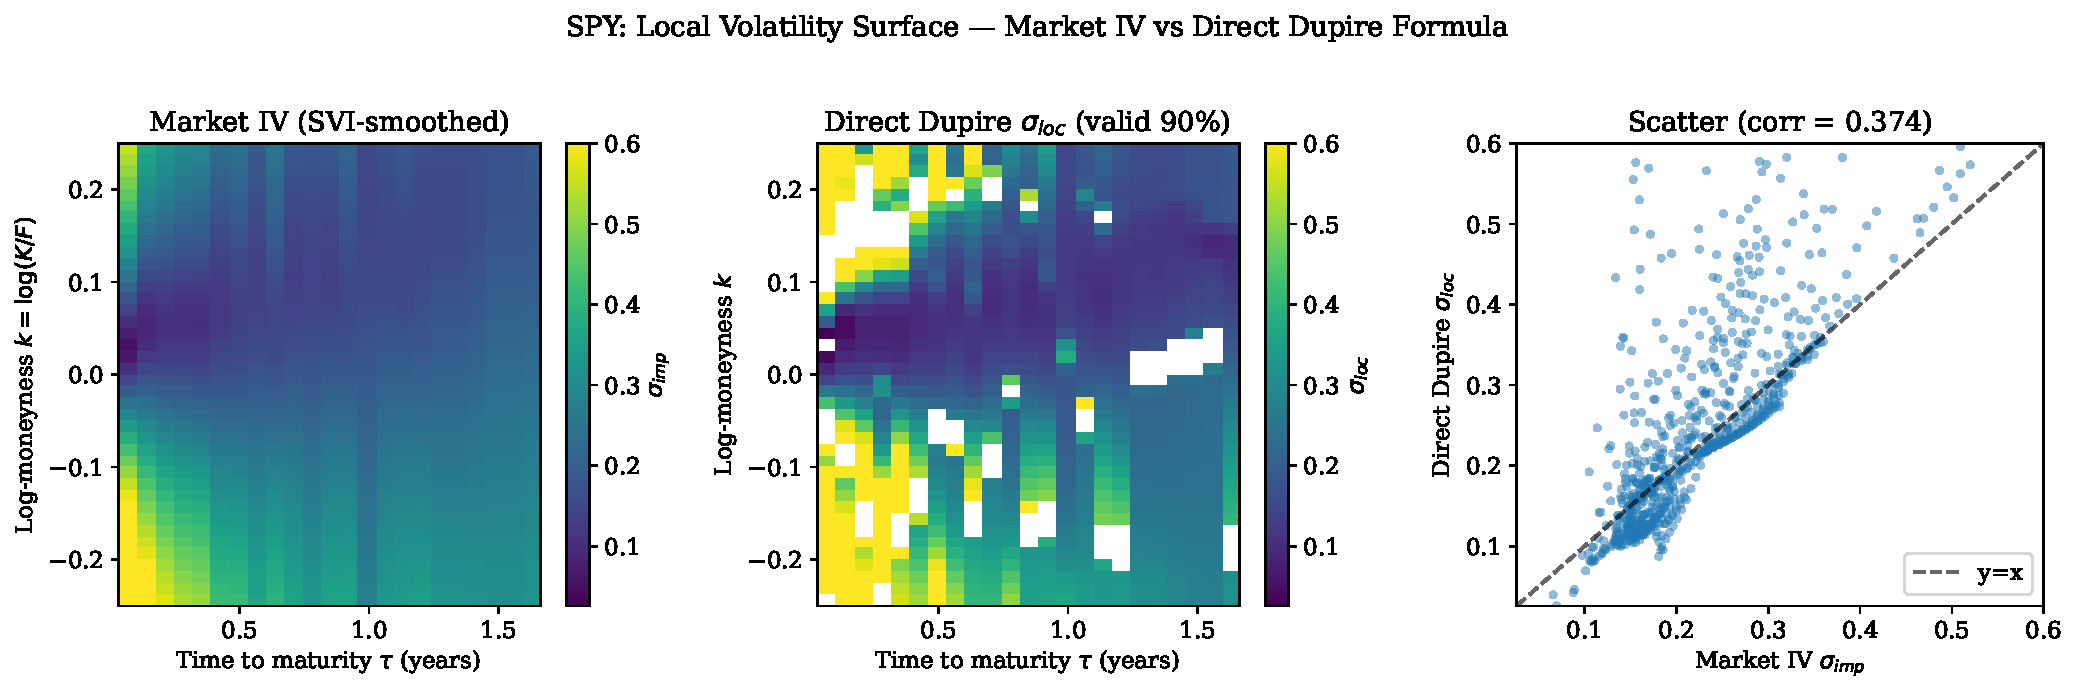
\includegraphics[width=\linewidth]{figures/local_vol_direct_vs_market_iv_SPY.pdf}
\caption{Direct Dupire formula $\sigma^2_{\text{loc}}{=}2(\theta+(r{-}q)K\partial_K C+qC)/(K^2\partial_{KK}C)$ on SPY using analytical $\theta$ (89.7\% of pixels valid, IV--vs--Dupire scatter correlation $0.37$).}
\end{figure}

\section{$[5,1]$ KAN in $(S,t)$ space and the 30-edge KAN}\label{app:5edge-kan}
A $[5,1]$ KAN trained in BS coordinates on the full library reaches test $R^2{=}0.510$ on real SPY (vs.\ $R^2{=}0.997$ on synthetic BS), with four of five activations nonlinear; the wider 30-edge KAN reaches $R^2{=}0.836$ but loses interpretability. Symbolic extraction from these activations is left to a follow-up manuscript; the $[2,1]$ KAN-Dupire in main-text \S3.2 is the maximally interpretable choice.

\section{SVI fitting and forward-price details}\label{app:svi}
SVI total variance $w(k){=}a+b(\rho(k{-}m)+\sqrt{(k{-}m)^2+s^2})$; converged on $100\%$ of $65$ expirations across the four tickers. Liquidity weights: $w_{\text{liq}}{\propto}\sqrt{\text{vol}\cdot\text{OI}}\cdot(1{+}\text{spread})^{-1}\cdot e^{-2k^2}$. Forward $F(\tau){=}S_0 e^{(r{-}q)\tau}$ with $q{\in}\{0.013, 0.005, 0.005, 0.007\}$ for SPY/QQQ/AAPL/MSFT.

\section{Out-of-sample analysis}\label{app:oos}
Trained on $\tau{<}0.5$ yr, evaluated on $\tau{\ge}0.5$ yr, the $[2,1]$ KAN-Dupire produces $R^2 \in \{-2.07, -2.57, -2.65, -1.11\}$ for SPY/QQQ/AAPL/MSFT --- the learned nonlinearity does not generalize across the term-structure dimension. Term-structure-aware operators are the natural next step.

\section{Computation costs}\label{app:cost}
\begin{table}[h]
\centering\footnotesize
\caption{Wall-clock per stage (s). Source: \texttt{computation\_costs.csv}.}
\begin{tabular}{lr}
\toprule
Stage & seconds \\
\midrule
Full pipeline & $1753.35$ \\
PINN training (all variants) & $473.18$ \\
\quad Original PINN (call+put) & $806.15$ \\
\quad Hard-constraint PINN & $283.34$ \\
\quad Log-price PINN & $270.36$ \\
Neural architecture sweep & $77.21$ \\
GP noise sweep (8 levels) & $11.30$ \\
Derivative-method comparison & $9.88$ \\
Ensemble SINDy & $0.032$ \\
Elastic Net & $0.083$ \\
PCA-SINDy & $0.017$ \\
\bottomrule
\end{tabular}
\end{table}

\section{$\sigma_{\text{SINDy}}$ vs.\ IV-averaging baselines}\label{app:sigma-cmp}
Volume-weighted IV achieves rel.\ error $\{0.3\%, 1.1\%, 5.0\%, 1.1\%\}$ on SPY/QQQ/AAPL/MSFT for ATM $\sigma$ recovery; median IV achieves $\{0.7\%, 4.5\%, 0.8\%, 4.8\%\}$; SINDy (linear Dupire) achieves $\{12.7\%, 10.6\%, 6.1\%, 29.3\%\}$. SINDy's value on real data is structural discovery and nonlinearity detection, not raw point-estimate accuracy. Source: \texttt{sigma\_method\_comparison.csv}.

\end{document}
